\documentclass[tikz,border=10pt]{standalone}
\usepackage{tikz}
\usetikzlibrary{shapes, arrows.meta, positioning, fit, calc, backgrounds, shadows}
\usepackage{amsmath, amssymb}
\usepackage{newtxtext,newtxmath}

%% ========== Color Definitions ==========
\definecolor{themeBlue}{RGB}{2, 119, 189}
\definecolor{themeGreen}{RGB}{0, 105, 92}
\definecolor{themeRed}{RGB}{183, 28, 28}

%% ========= TikZ Styles ==========
\tikzset{
    node distance=1.5cm and 2cm, % 设置默认的节点间距
    font=\footnotesize\sffamily,
    %
    % 基础节点样式
    baseBlock/.style={
        rectangle, thick, rounded corners=2pt,     
        minimum width=2cm, minimum height=1cm, 
        align=center,                              
        drop shadow={opacity=0.08, shadow xshift=1pt, shadow yshift=-1pt} 
    },
    %
    A/.style={baseBlock, draw=themeBlue, fill=themeBlue!10},   
    B/.style={baseBlock, draw=themeGreen, fill=themeGreen!10}, 
    C/.style={baseBlock, draw=themeRed, fill=themeRed!10},     
    %
    % 连线样式
    conn/.style={
        draw=black!70, 
        line width=0.8pt,
        -{Latex[length=2.5mm, width=1.5mm]} % arrows.meta 库的精致箭头
    },
    %
    % 印章：电脑
    pcStamp/.pic={
        \begin{scope}[scale=0.6, thick, draw=black!70]
            \filldraw[fill=white] (-1.2, -0.8) rectangle (1.2, 0.8); % 背景色块（带边框）
            \fill[themeBlue!10] (-1.0, -0.6) rectangle (1.0, 0.6);   % 图形色块
            \draw (0, -0.8) -- (0, -1.3);
            \draw (-0.7, -1.3) -- (0.7, -1.3);
            \node[text=themeBlue, xshift=15pt, yshift=-6pt] at (0, 0) {WORK};
        \end{scope}
    },
    %
    % 印章：小人
    stickman/.pic={
        \begin{scope}[scale=0.5, thick, draw=black!80]
            \draw (0, 0.6) circle (0.3);        % 头
            \draw (0, 0.3) -- (0, -0.6);        % 身体
            \draw (-0.5, 0.1) -- (0.5, 0.1);    % 胳膊
            \draw (0, -0.6) -- (-0.4, -1.3);    % 左腿
            \draw (0, -0.6) -- (0.4, -1.3);     % 右腿
        \end{scope}
    }
}

\begin{document}
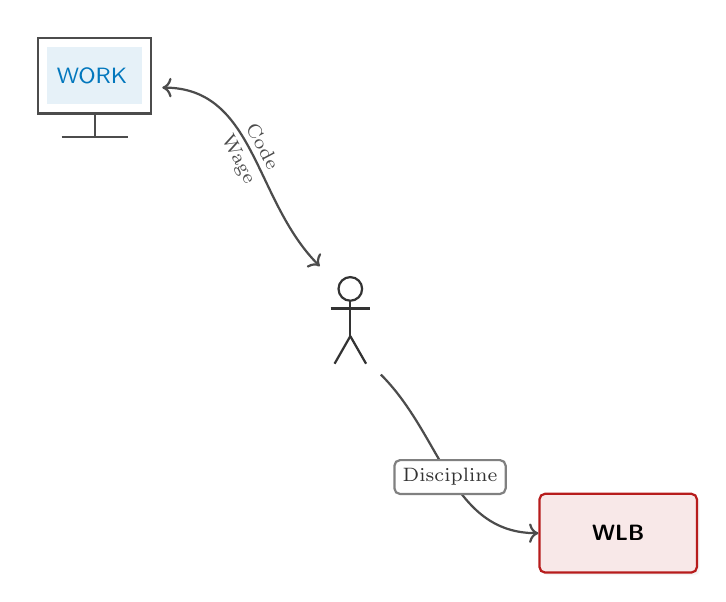
\begin{tikzpicture}

	%% 布局
	\node (man) at (0,0) {\tikz\pic{stickman};};    % node 声明 + (标签) + at (绝对中心位置) + {内容}
	\node (pc) [above left=of man] {\tikz\pic{pcStamp};}; % node 声明 + (标签) + [相对位置] + {内容}
	\node (wlb) [C, below right=of man] {\textbf{WLB}};

	%% 连线 \draw[样式] (起点) -- 途中节点 (终点);
	\draw[conn, <->] (pc.east) to [out=0, in=135]
	node [above, sloped, inner sep=2pt, font=\scriptsize, text=black!70] {Code}
	node [below, sloped, inner sep=2pt, font=\scriptsize, text=black!70] {Wage}
	(man.north west);

	% 从“人”通往“WLB”的曲线上，横亘着：Discipline
	\draw[conn, ->] (man.south east) to [out=-45, in=180]
	node [draw=black!50, fill=white, rectangle, rounded corners=2pt, thick, font=\scriptsize, text=black!80, inner sep=3pt] {Discipline}
	(wlb.west);

\end{tikzpicture}
\end{document}